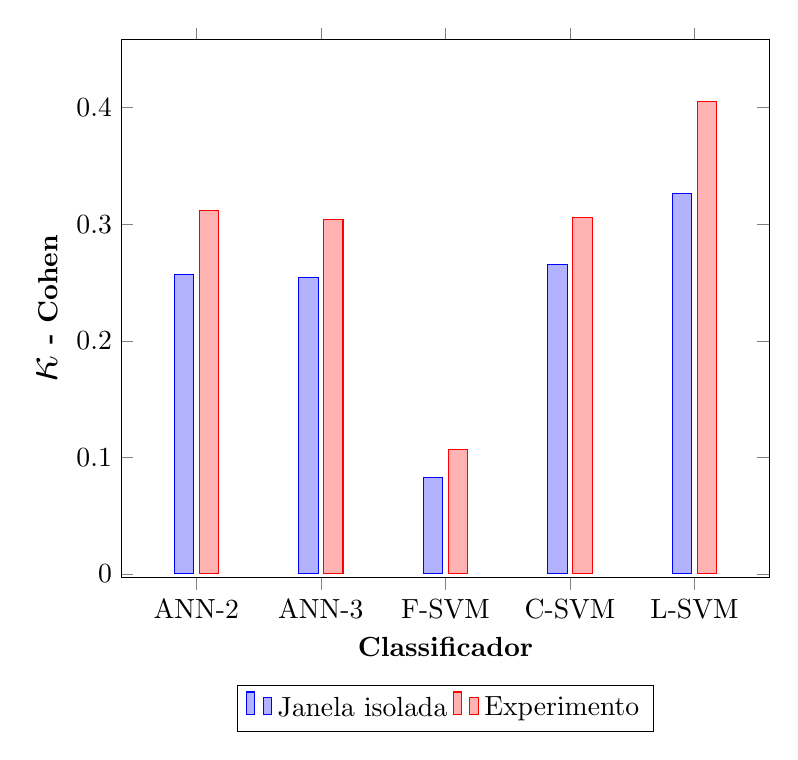
\begin{tikzpicture}
\begin{axis}[ybar,
ylabel={\textbf{{\LARGE $\kappa$} - Cohen}},
symbolic x coords={ANN-2,ANN-3,F-SVM,C-SVM,L-SVM},
enlargelimits=0.15,
bar width=7pt,
xlabel={\textbf{Classificador}},
xtick=data,
legend style={at={(0.5,-0.2)},anchor=north,legend columns=-1},
scale=1.2,
ymin=0.05,
]
\addplot coordinates {
	(ANN-2,0.256710322461084)
	(ANN-3,0.253969286000733)
	(F-SVM,0.08251886405747)
	(C-SVM,0.265203892414323)
	(L-SVM,0.32674780825939)
};
\addplot coordinates {
	(ANN-2,0.311612621296827)
	(ANN-3,0.304360005958168)
	(F-SVM,0.106615596193986)
	(C-SVM,0.305949166653495)
	(L-SVM,0.405089519212324)
};
\legend{Janela isolada,Experimento}
\end{axis}
\end{tikzpicture}